\documentclass[letterpaper]{article}
\usepackage[submission]{aaai2027}
\usepackage{tikz}
\usetikzlibrary{arrows.meta, positioning, calc}
\frenchspacing
\setcounter{secnumdepth}{2}

\title{tikz test}
\author{x}
\affiliations{x}

\tikzset{
  ag/.style   = {circle, draw, minimum size=7mm, inner sep=0pt, font=\scriptsize, align=center},
  dec/.style  = {ag, very thick, fill=black!10},
  flow/.style = {-{Latex[length=2mm]}, draw=black!55},
  lever/.style= {-{Latex[length=2.6mm]}, very thick, draw=orange!85!black},
  xin/.style  = {-{Latex[length=1.6mm]}, draw=black!45, dashed},
  ttl/.style  = {font=\footnotesize\bfseries},
  sub/.style  = {font=\scriptsize, text=black!70},
  lev/.style  = {font=\scriptsize\itshape, text=orange!60!black}
}

\begin{document}
\maketitle

\begin{figure*}[t]\centering
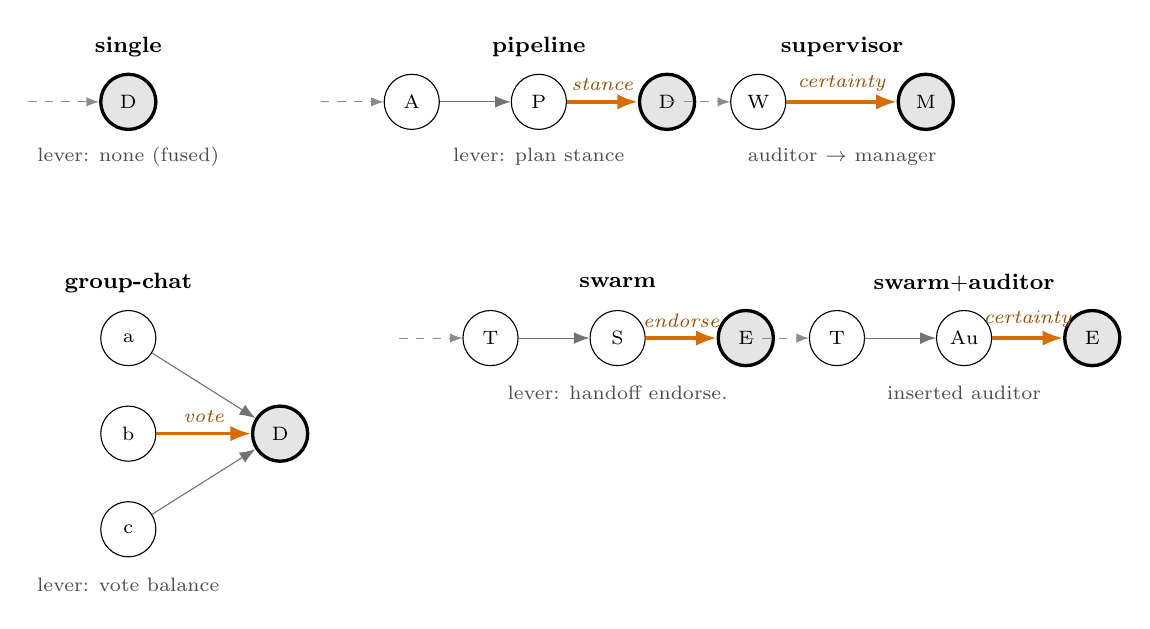
\begin{tikzpicture}[node distance=8mm and 9mm]
%% ===== top row =====
% (1) single
\begin{scope}[local bounding box=A]
  \node[dec] (d1) {D};
  \draw[xin] ([xshift=-9mm]d1.west) -- (d1);
  \node[ttl] at ([yshift=7mm]d1) {single};
  \node[sub] at ([yshift=-7mm]d1) {lever: none (fused)};
\end{scope}
% (2) pipeline
\begin{scope}[shift={(3.6,0)}, local bounding box=B]
  \node[ag] (a2) {A};
  \node[ag, right=of a2] (p2) {P};
  \node[dec, right=of p2] (d2) {D};
  \draw[xin] ([xshift=-8mm]a2.west) -- (a2);
  \draw[flow] (a2) -- (p2);
  \draw[lever] (p2) -- node[lev, above]{stance} (d2);
  \node[ttl] at ([yshift=7mm]p2) {pipeline};
  \node[sub] at ([yshift=-7mm]p2) {lever: plan stance};
\end{scope}
% (3) supervisor (the main edge)
\begin{scope}[shift={(8.0,0)}, local bounding box=C]
  \node[ag] (w3) {W};
  \node[dec, right=14mm of w3] (m3) {M};
  \draw[xin] ([xshift=-8mm]w3.west) -- (w3);
  \draw[lever] (w3) -- node[lev, above]{certainty} (m3);
  \node[ttl] at ([yshift=7mm]$(w3)!0.5!(m3)$) {supervisor};
  \node[sub] at ([yshift=-7mm]$(w3)!0.5!(m3)$) {auditor $\to$ manager};
\end{scope}
%% ===== bottom row (y = -3) =====
% (4) groupchat
\begin{scope}[shift={(0,-3)}, local bounding box=D]
  \node[ag] (g1) {a};
  \node[ag, below=5mm of g1] (g2) {b};
  \node[ag, below=5mm of g2] (g3) {c};
  \node[dec, right=12mm of g2] (d4) {D};
  \draw[flow] (g1) -- (d4);  \draw[flow] (g3) -- (d4);
  \draw[lever] (g2) -- node[lev, above]{vote} (d4);
  \node[ttl] at ([yshift=7mm]g1) {group-chat};
  \node[sub] at ([yshift=-7mm]g3) {lever: vote balance};
\end{scope}
% (5) swarm
\begin{scope}[shift={(4.6,-3)}, local bounding box=E]
  \node[ag] (t5) {T};
  \node[ag, right=of t5] (s5) {S};
  \node[dec, right=of s5] (e5) {E};
  \draw[xin] ([xshift=-8mm]t5.west) -- (t5);
  \draw[flow] (t5) -- (s5);
  \draw[lever] (s5) -- node[lev, above]{endorse} (e5);
  \node[ttl] at ([yshift=7mm]s5) {swarm};
  \node[sub] at ([yshift=-7mm]s5) {lever: handoff endorse.};
\end{scope}
% (6) swarm + auditor (causal probe)
\begin{scope}[shift={(9.0,-3)}, local bounding box=F]
  \node[ag] (t6) {T};
  \node[ag, right=of t6] (au6) {Au};
  \node[dec, right=of au6] (e6) {E};
  \draw[xin] ([xshift=-8mm]t6.west) -- (t6);
  \draw[flow] (t6) -- (au6);
  \draw[lever] (au6) -- node[lev, above]{certainty} (e6);
  \node[ttl] at ([yshift=7mm]au6) {swarm$+$auditor};
  \node[sub] at ([yshift=-7mm]au6) {inserted auditor};
\end{scope}
\end{tikzpicture}
\caption{MAS topologies. Shaded node = the \emph{decider} that authorizes the action; the thick orange edge
carries that topology's \emph{lever} (the upstream content the decider defers to). Dashed = attacker entry point.}
\end{figure*}

\end{document}
